% Report-ExperimentalRelaxationInvestigations.tex
% Simon Hulse
% simonhulse@protonmail.com
% Last Edited: Wed 27 Nov 2024 02:43:47 PM EST

% !TeX root = ./Report-Body.tex
\chapter{Experimental Relaxation Investigations}
In an attempt to gain an in-depth understanding of methyl relaxation, a series of NMR experiments were conducted on a test compound over a range of temperatures. By varying temperature, the viscosity of the medium in the NMR tube changes. As such, doing this provides a means of monitoring relaxation rates as function of rotational correlation time, $\tau_{\text{c}}$. The molecule considered in these studies is shown in Figure \ref{TransverseSpectra}. This was present in a highly viscous medium composed of $95 \%$ d-glycerol and $5 \%$ d-DMSO. The intention was for this simple, small molecule to mimic the motional behaviour typical of molecules far larger that it.
\section{Experiments Conducted}
Transverse $^{13}$C relaxation experiments were carried out to determine the four rates, $\Gamma_{2,\text{C}}^{i}$ (discussed in the previous chapter), experimentally. Furthermore, $^1$H translational diffusion experiments were conducted, which can be used as a gauge of the molecule's motional behaviour. All Experiments were carried out on a Varian $\num{600} \si{\mega \myhertz}$ spectrometer. Spectra were processed using NMRPipe\cite{RN43}.\\
\subsection{$^{13}$C Transverse Relaxation Experiment}
\begin{figure}
\centering
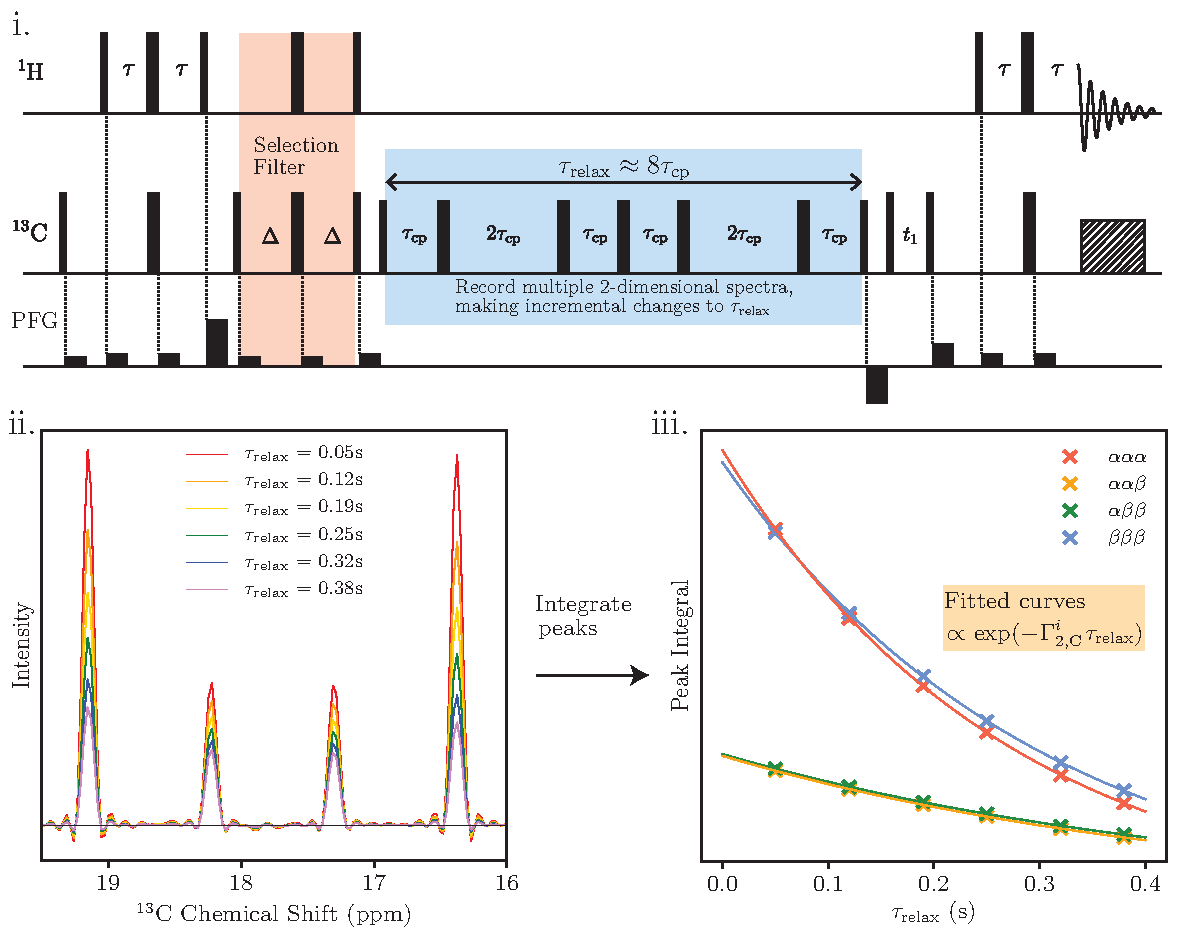
\includegraphics[scale=0.75]{./Figures/SimonsFigs/DecayCurves.pdf}
\caption{i. The pulse sequence used to determine $^{13}$C transverse relaxation rates. ii. A cross section through a $^{13}$C quartet, of two-dimensional spectra obtained using the pulse sequence. As $\tau_{\text{relax}}$ is increased, the intensity of the peaks in the quartet decreases. Individual peaks in each spectrum are integrated, and these integrals are plotted as a function of $\tau_{\text{relax}}$, iii. Fitting exponential curves to each set of points allows extraction of relaxation rates of each coherence at a given temperature. The experiment is then repeated using a range of temperatures to determine how relaxation rates vary with viscosity.}
\label{RelaxDecay}
\end{figure}
The acquisition of experimental values for $\Gamma_{2,S}^i$ was achieved using the pulse sequence in Figure \ref{RelaxDecay}.i. $^{13}$C single-quantum coherences were generated via use of an INEPT sequence\cite{RN54}, and subsequently allowed to evolve for a specified period of time, $\tau_{\text{relax}}$. The pulse sequence used has many similarities with a conventional HSQC pulse sequence, shown in Figure \ref{HSQCHMQC}.ii. Two major elements are added to the sequence, enabling relaxation rate studies:
\begin{itemize}
\item A selection filter (highlighted in red), devised by Kontaxis and Bax\cite{RN3}. Varying the value of the time delay $\Delta$, and taking linear combinations of spectra enables the isolation of a single peak within the methyl quartet.
\item A Carr-Purcell-Meiboom-Gill (CPMG) element\cite{RN47,RN48} (highlighted in blue), during which the desired coherences are allowed to relax.
\end{itemize}
By obtaining a series of spectra\footnote{The spectra in Figure \ref{RelaxDecay}.ii. adopt an approximate intensity ratio of 3:1:1:3, at least for smaller $\tau_{\text{relax}}$ values. This contrasts with what is typical of a 1D $^{13}$C spectrum, where a 1:3:3:1 intensity ratio results. This intensity ratio manifests as a result of the way the magnetisation evolves during the HSQC pulse sequence\cite{RN49}} with differing values of $\tau_{\text{relax}}$, and integrating the resultant peaks, a decay profile is obtained. The relaxation rate of each coherence is calculated by fitting an exponential function to the decay profile. Repetitions of this experiment were then carried out, at different temperatures.\\
\begin{figure}
\centering
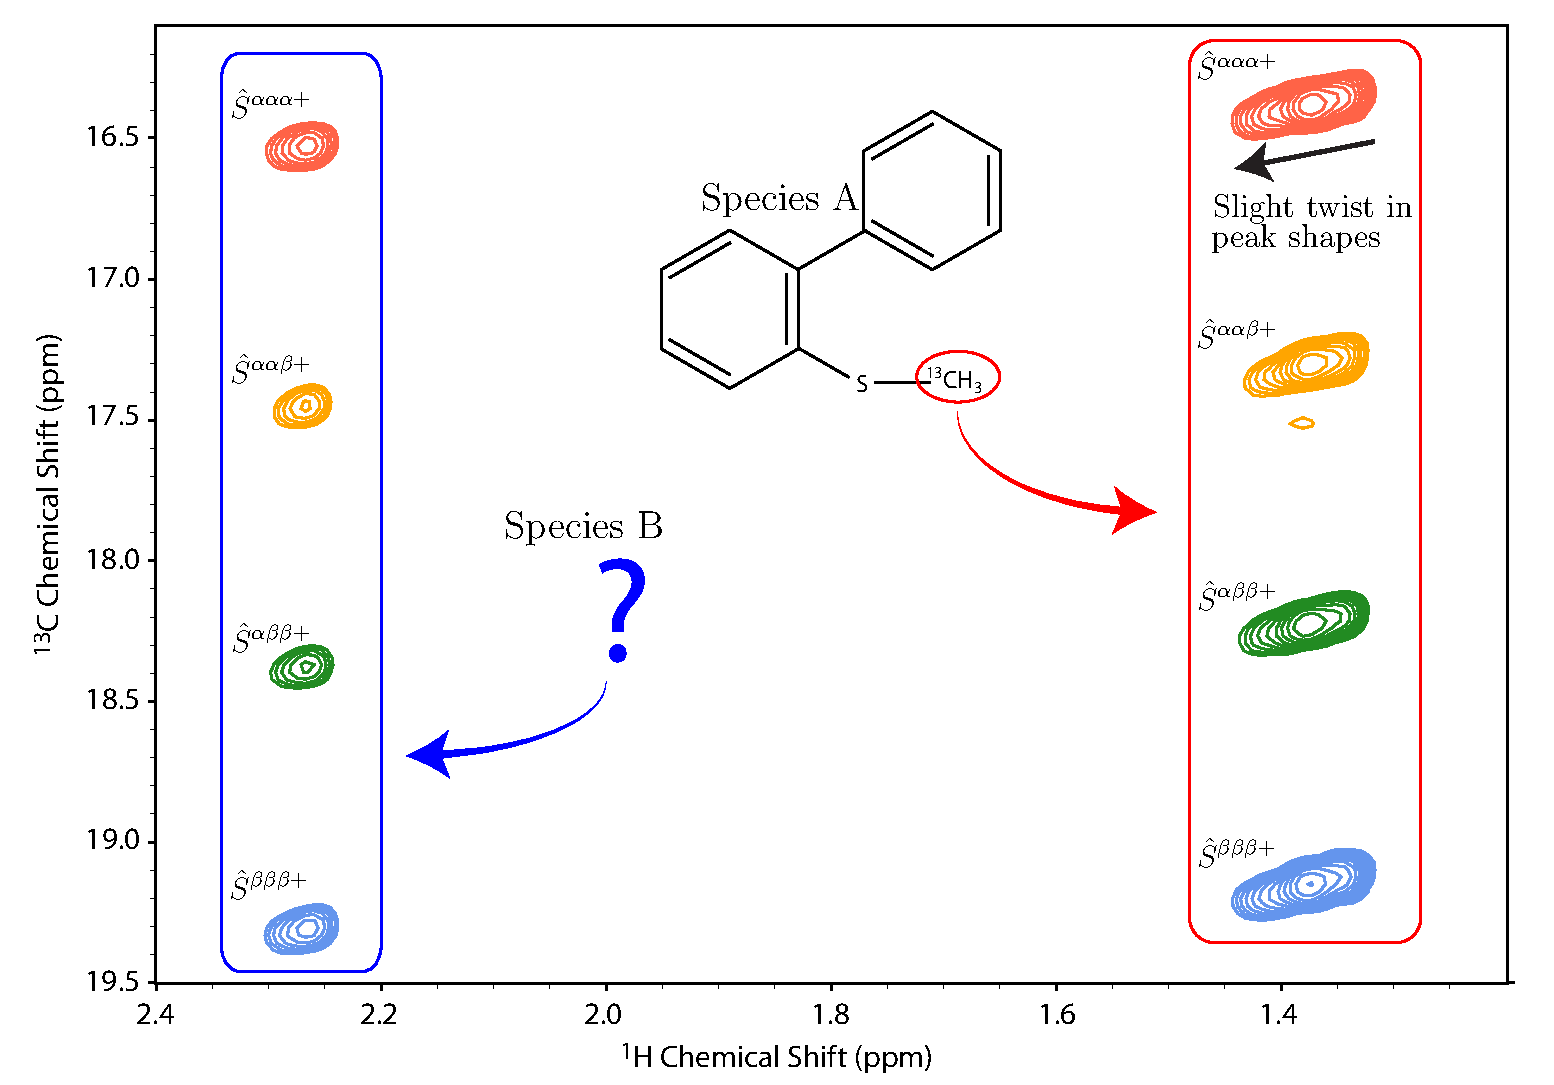
\includegraphics[scale=0.5]{./Figures/SimonsFigs/13CTransExptSpectrum.pdf}
\caption{An example of a spectrum obtained using the $^{13}$C transverse relaxation experiment. The spectrum were taken at $T = \num{30}^{\circ}\text{C}$, with $\tau_{\text{relax}} = \num{0.05} \si{\second}$. Two distinct chemical environments are present in the spectrum, indicating two species, A and B, are present.}
\label{TransverseSpectra}
\end{figure}
Figures \ref{TransverseSpectra} shows an example spectrum obtained using the $^{13}$C transverse relaxation experiment. The expected spectrum of a molecule with one $^{13}$CH$_3$ moiety is a single quartet. Curiously, the spectra obtained instead comprised two separate quartets. The implication of this is that two distinct chemical species, each possessing $^{13}$CH$_3$ moieties, were present in the sample (which will be referred to as A and B). This was a rather fortuitous outcome, as it enabled the acquisition of a larger data set.\\
The peak shapes exhibited a slightly twisted geometry in the spectra, as is indicated in Figure \ref{TransverseSpectra}, which was probably due to isotope-shift effects.\\
\subsection{Diffusion Experiments}
Diffusion NMR experiments measure the attenuation of a sample's signal, via the application of pulsed field gradients (PFGs)\cite{RN51}. Larger molecules, which translate slowly in solution, suffer less signal attenuation with increasing gradient strength, relative to smaller, more rapidly translating molecules. Measuring signal intensity as a function of gradient strength, and fitting the data using the Stejskal-Tanner equation\cite{RN42} provides a means of determining the translational diffusion constant, $D$, of the various species in an NMR sample.\\
1D proton diffusion experiments were conducted on the sample, at varying temperatures. It was possible to determine translational diffusion constants for both species A and B. As well as this, diffusion data for the glycerol could also be obtained.
\section{Fitting Relaxation Models to the Data}
The ability of the Woessner and diffusive models to describe the data was assessed using a least squares fitting procedure. The solution of a least squares procedure is that which minimises the summation of squared residuals, commonly denoted $\chi^2$:
\begin{equation}
\chi^2 = \sum \limits_i (y_{i,\text{data}} - y_{i,\text{fit}})^2
\end{equation}
A least squares procedure to globally optimise the parameters $\Delta \sigma_{\text{I}}$, $\Delta \sigma_{\text{S}}$ and $\tau_{\text{m}}$ was performed, using both the Woessner and diffusive models. To incorporate the effect of external protons in the molecule into the fit, it was assumed that a single proton existed, separated from the methyl protons by a distance $r_{\text{ext}}$. The value of $r_{\text{ext}}$ was also included in the fitting procedure. On top of globally fitting the aforementioned parameters, $\tau_{\text{c}}$ was optimised at each temperature (locally). Fits in which $\tau_{\text{m}}$ were set to be local were also carried out. It was found that the $\chi^2$ values of fits incorporating local and global $\tau_{\text{m}}$ were very similar, which lead to the decision to fit it globally. One major difference between the Woessner and diffusive models is the temperature dependence of methyl rotation. In the Woesnner model, the protons undergo activationless jumps, and hence exhibit no temperature dependence. Conversely $\tau_{\text{m}}$ is anticipated to vary with temperature if the diffusive model is obeyed, as an activation barrier to the motion is present. The lack of any significant local dependence of $\tau_{\text{m}}$ is evidence in favour of the Woessner model.\\
In order to determine errors for the fitting parameters, a bootstrapping method was applied. This method relies on taking a random sample of data points from the complete data set, allowing repetition of points, and performing the same optimisation procedure again. This process is then repeated multiple times. In the limit of infinite runs, it is anticipated that the mean of the distribution of values determined for a particular parameter will converge on its true value. The standard deviation in values of the bootstrap acts as measure of the error in the fitting parameter.
\subsection{Species A}
\begin{figure}
\centering
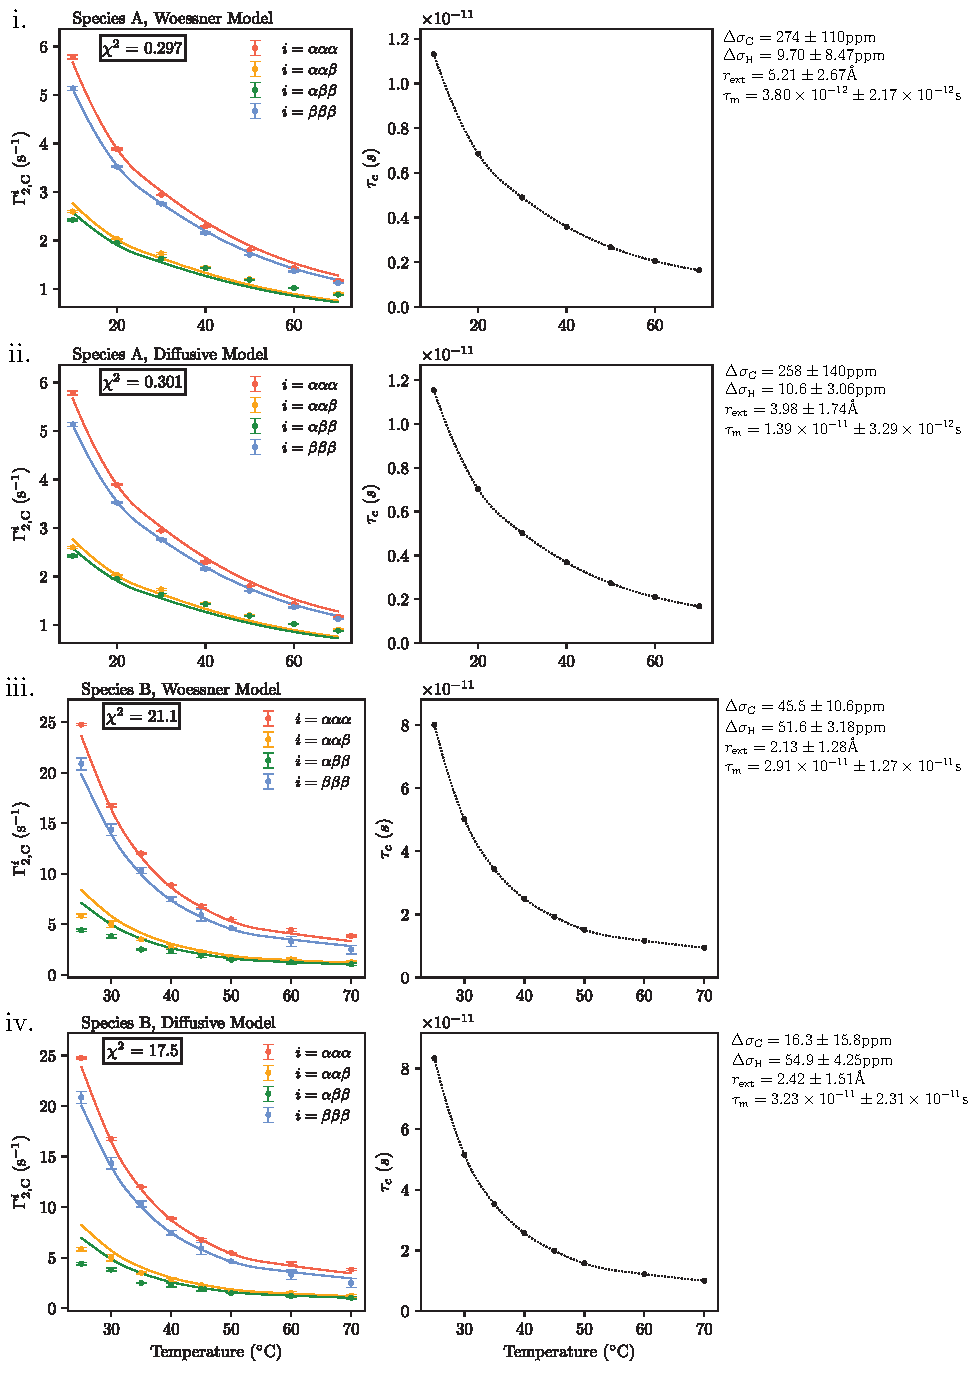
\includegraphics[scale=0.9]{./Figures/SimonsFigs/Fits.pdf}
\caption{Results of a least squares fitting procedure, using both the Woessner and diffusive models, applied to the $^{13}$C transverse relaxation rate data acquired.}
\label{Fits}
\end{figure}
Plots i. and ii. in Figure \ref{Fits} show the results of the least squares procedure applied to species A, using both the Woessner and diffusive models. The $\chi^2$ values obtained show a close agreement between the models. Also, the values of the fitted parameters were found to be highly similar. This meant there was very little scope to compare the two models. The $\tau_{\text{{c}}}$ values obtained imply that the molecule is undergoing rapid tumbling, and is certainly not adhering in the macromolecular limit. The $^{13}$C CSA is predicted to be very large by the fitting procedure. Typical methyl $^{13}$C CSA values are between 17-25ppm, for Ile and Val\cite{RN50}. Though this may be anticipated to be slightly higher when the methyl group is adjacent to a sulfur atom, an increase of 2 orders of magnitude is unlikely.  Plots i. and ii. in Figure \ref{CH3Models} provide predictions of relaxation rates made by the models, using parameters which are typical for a methyl moiety. It can be seen that the relaxation rates of the two outer ($\alpha \alpha \alpha$ and $\beta \beta \beta$) lines are virtually identical in the fast tumbling regime. Despite this, noticeable differences are observed in the acquired data. The fitting procedure has accounted for this split in the rates by setting $\Delta \sigma_{\text{C}}$ to be very large.
\subsection{Species B}
The analogous results of the fitting procedure for species B are shown in iii. and iv. of Figure \ref{Fits}. In this case, the diffusive model did seem to produce a slightly better fit, relative to the Woessner model, though again, the difference was very minor.
\section{Comparing Diffusion Data with Relaxation Data}
Predictions of the hydrodynamic radii, $r_{\text{H}}$, of the species were carried out, by implementation of the Stokes-Einstein equation:
\begin{equation}
\label{Stokes}
r_{H} = \frac{k_{\text{B}}T}{6\pi \eta D}
\end{equation}
where $k_{\text{B}}$ is the Boltzmann constant, and $\eta$ is the viscosity of the medium. The viscosity of the medium was calculated over the range of temperatures considered, by use of an empirically determined model, and assuming the medium was comprised of pure glycerol\cite{RN52}.\\
\begin{figure}
\centering
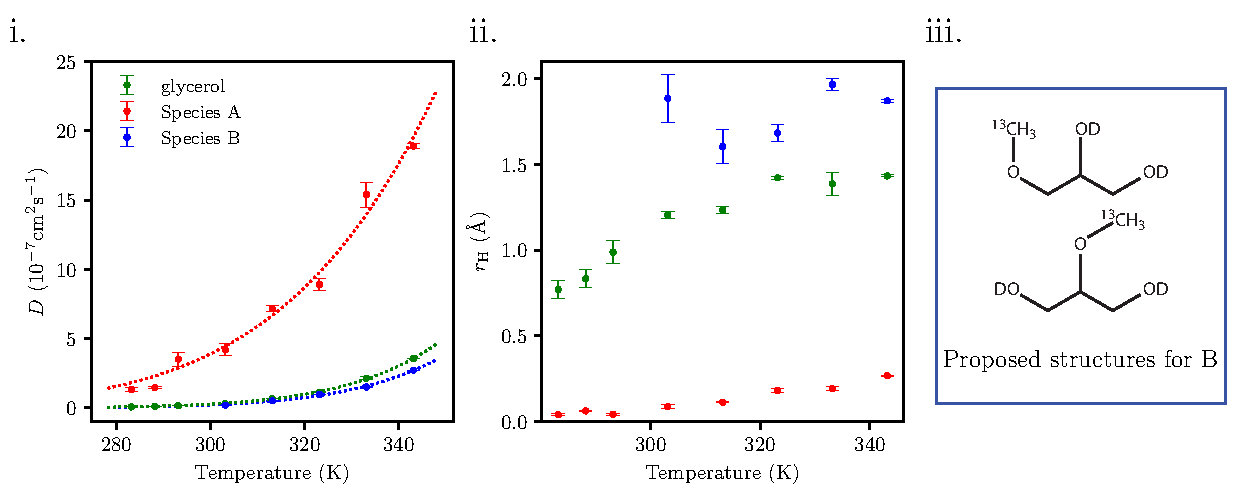
\includegraphics[scale=0.7]{./Figures/SimonsFigs/Diffusion.pdf}
\caption{i. Plots of translational diffusion constant, $D$, versus temperature for species A, species B, and glycerol. Arrhenius-type fits of the form $D = A\exp(-\frac{B}{T})$ were generated for each species. ii. Calculated hydrodynamic radii, $r_{\text{H}}$, for the three species as a function of temperature. iii. By noting that the diffusion constants of species B and glycerol are very closely matched, it is proposed that either of the structures shown could correspond to species B.}
\label{Diffusion}
\end{figure}
From the data in Figure \ref{Diffusion}.i., species A was found to be diffusing far more rapidly than both the glycerol and species B. This implies that species A is able to translate in an unrestricted fashion, without too much hindrance from the viscous medium it is in. The hydrodynamic radii across all temperatures were calculated to be on the order of $\num{E-11} \si{\meter}$, which is far smaller than anticipated for a molecule of its size. On account of this, along with the very small rotational correlation times predicted from the relaxation rate fits, it is postulated that the molecule is diffusing through the medium in a highly anisotropic, 'bullet-like' fashion, as would be expected of a prolate spheroid.\\
In order to assess this prediction, the rotational correlation times extracted from our fitted Woessner model was compared with the hydrodynamic data obtained of species A. The following expression relates the rotational correlation time with the hydrodynamic radius of the molecule\cite{RN56}:
\begin{equation}
\label{TaucRH}
\tau_{\text{c}} = \lambda\frac{4 \pi \eta r_{\text{H}}^3}{3k_{\text{B}}T}
\end{equation}
$\lambda$ is a constant that indicates deviation from spherical behaviour. For a perfect sphere, it is predicted that $\lambda = 1$. Using \ref{Stokes} and \ref{TaucRH}, the following expression for $\lambda$ can be obtained, in terms of the hydrodynamic radius of glycerol, and the diffusion constants of glycerol and species A:
\begin{equation}
\lambda = \frac{4 r_{\text{H,gly}}^2 D_{\text{gly}}^2}{18D_{\text{A}}^3}
\end{equation}
A plot of $\lambda$ versus temperature is shown in Figure \ref{Lambda}. The values of $\lambda$ show a decline with temperature, but for the most part they are comfortably above 1, which acts to validate the proposal that the molecule is not undergoing spherical motion.
\begin{figure}
\centering
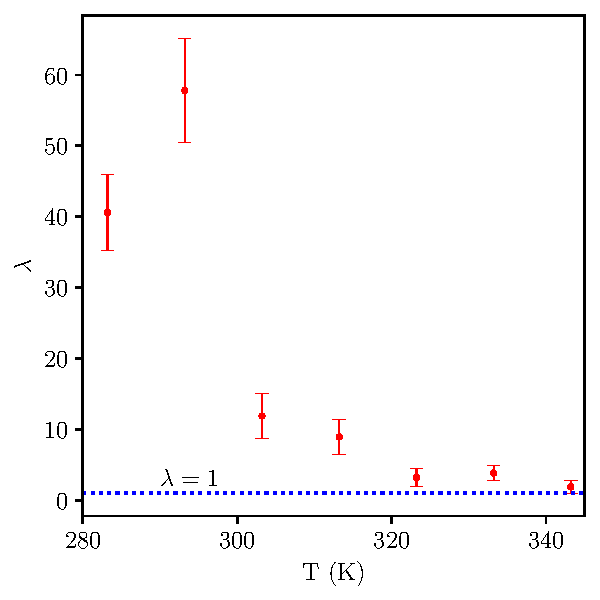
\includegraphics[scale=0.7]{./Figures/SimonsFigs/Lambda.pdf}
\caption{A plot of $\lambda$ versus $T$ for species A. A decline in the value of $\lambda$ is found with increasing temperature, indicating that the molecule's motion is becoming less anisotropic as the viscosity of glycerol decreases.}
\label{Lambda}
\end{figure}
Figure \ref{AnisotropicMotion} illustrates how we anticipate this molecule behaves within the medium. First, it is able to translate far more effectively in one dimension that the other two, following a largely linear path. As well as this, the global rotation of the molecule about its major axis is less hindered by the medium, relative to rotation about its other axes. In order to effectively account for anisotropic tumbling, it would be necessary to redefine the spectral density function which describes the global motion. Accounts of spectral densities for anisotropic motions are well documented in the literature, with the relevant expression for a prolate spheroid being the following\cite{RN53}:
\begin{equation}
J(\omega) = \frac{1}{4}\left(3\cos^2\theta-1\right)^2 \frac{\tau_{\text{A}}}{1+ \omega^2\tau_{\text{A}}^2} + 3\sin^2\theta\cos^2\theta \frac{\tau_{\text{B}}}{1+ \omega^2\tau_{\text{B}}^2} + \frac{3}{4}\sin^4\theta\frac{\tau_{\text{C}}}{1+ \omega^2\tau_{\text{C}}^2}
\end{equation}
with the correlation times $\tau_{\text{A}}, \tau_{\text{B}}, \tau_{\text{C}}$ depending on the rotational diffusion constants perpendicular and parallel to the spheroid's axis of symmetry ($D_{\perp}$ and $D_{\parallel}$). It is highly plausible that an additional component of motion is also in effect: the rotation of the methyl threefold axis, characterised by correlation time $\tau_{\text{axis}}$. As mentioned earlier in this thesis, this motion has been incorporated into relaxation models via a model-free approach\cite{RN31}.\\
\begin{figure}
\centering
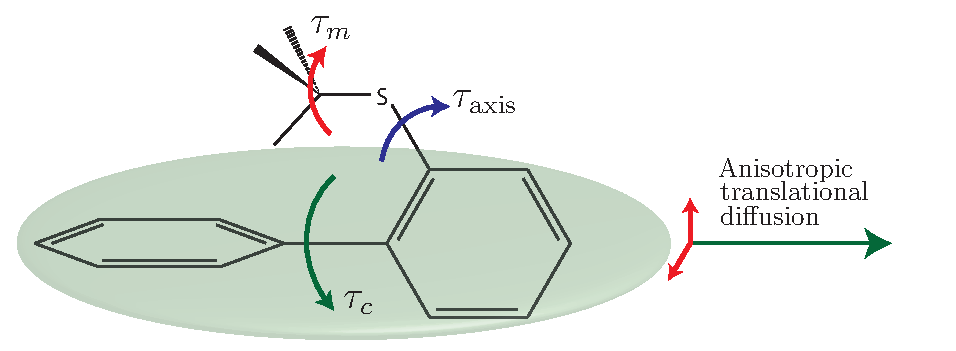
\includegraphics[scale=0.8]{./Figures/SimonsFigs/SpeciesAMotion.pdf}
\caption{The proposed types of motion adopted by species A within the glycerol medium. Anisotropic translational and rotational diffusion are both acting, as would be expected of a prolate spheroid. The uncorrelated motion of the methyl symmetry axis may also feature.}
\label{AnisotropicMotion}
\end{figure}
Species B exhibits very similar diffusion properties to glycerol, as seen in Figure \ref{Diffusion}. This provides evidence that species B is formed as the product of a reaction between glycerol and species A. Potential structures of species B, which fit this hypothesis are shown in Figure \ref{Diffusion} iii., though further studies to gain clarity on this matter were not carried out.
\section{Summary of Experimental Results}
The results obtained from fitting our models show that our theory is able to describe the $^{13}$C relaxation rate data effectively. The temperature independence of $\tau_{\text{m}}$ that is observed from the fitting procedure points to the Woessner model as the more effective of the two at describing methyl relaxation phenomena. The test molecule, which was hoped to mimic proteins by being present in a highly viscous medium, never left the small molecules limit. This is accounted for by noting it travelled in a highly anisotropic, 'bullet-like' fashion. The motion became more isotropic as the viscosity of the glycerol increased, as evidenced by a decrease in $\lambda$ with temperature.
